


%-----------------------------------------------------------------------------------------%
%-----------------------------------------------------------------------------------------%


\chapter{Introduction}

\section{Sex Differences in Mortality and Health}

\subsection{Gaps in Life Expectancy Between Men and Women}

A female advantage in life expectancy has been reported for most 
historic populations, even when levels of maternal mortality were 
high.\citep{klasen1998marriage,mcnay2005excess,zarulli2018women} 
Before the 19th century, sex differences in life expectancy were 
generally small as poor living conditions, inadequate sanitation, 
epidemics, and famines resulted in high levels of mortality among 
both men and women.\citep{thorslund2013} Throughout the 19th and 
20th centuries, the impact of these external hazards diminished. 
At the same time, the impact of infectious diseases rapidly decreased 
and non-communicable diseases became the major causes of death, 
including cardiovascular diseases and neoplasms. This process is 
known as the epidemiological transition.\citep{omran1971epidemiologic,
blacher2016epidemiological}

Key features of the epidemiological transition were sustained 
improvements in life expectancy for men and women in most developed 
countries.\citep{christensen2009ageing} Following this modern mortality 
decline, but with a lag of about half a century, sex differences 
in life expectancy started to widen. While differences in life 
expectancy between men and women widened slowly during the 19th century, 
they increased more rapidly throughout the 20th century as mortality 
became increasingly patterned by behavioral factors.\citep{vallin2004convergences,gjonca2005} 
In nearly all developed countries, sex differences in life expectancy 
peaked in the 1970s and 1980s and declined thereafter.\citep{glei2007narrowing,clark2012examining} 
Today, women outlive men in all countries of the world.\citep{barford2006life,desa2017world}

\hyperref[ch1:fig1]{Figure 1} illustrates the magnitude of sex differences in 
life expectancy at birth. Women's advantage in life expectancy is shown for 
Denmark and all other countries covered in the Human Mortality Database (HMD).\citep{human2005university} 
An important feature to highlight is that the magnitude of women's advantage 
in life expectancy has varied over time, and even differs in developed countries 
today. For example, in 2016, women had an advantage of 3.6 years in Iceland 
and 10.1 years in Belarus.\citep{human2005university} \\


	%------------------%
	\begin{figure}[H]
		\centering
		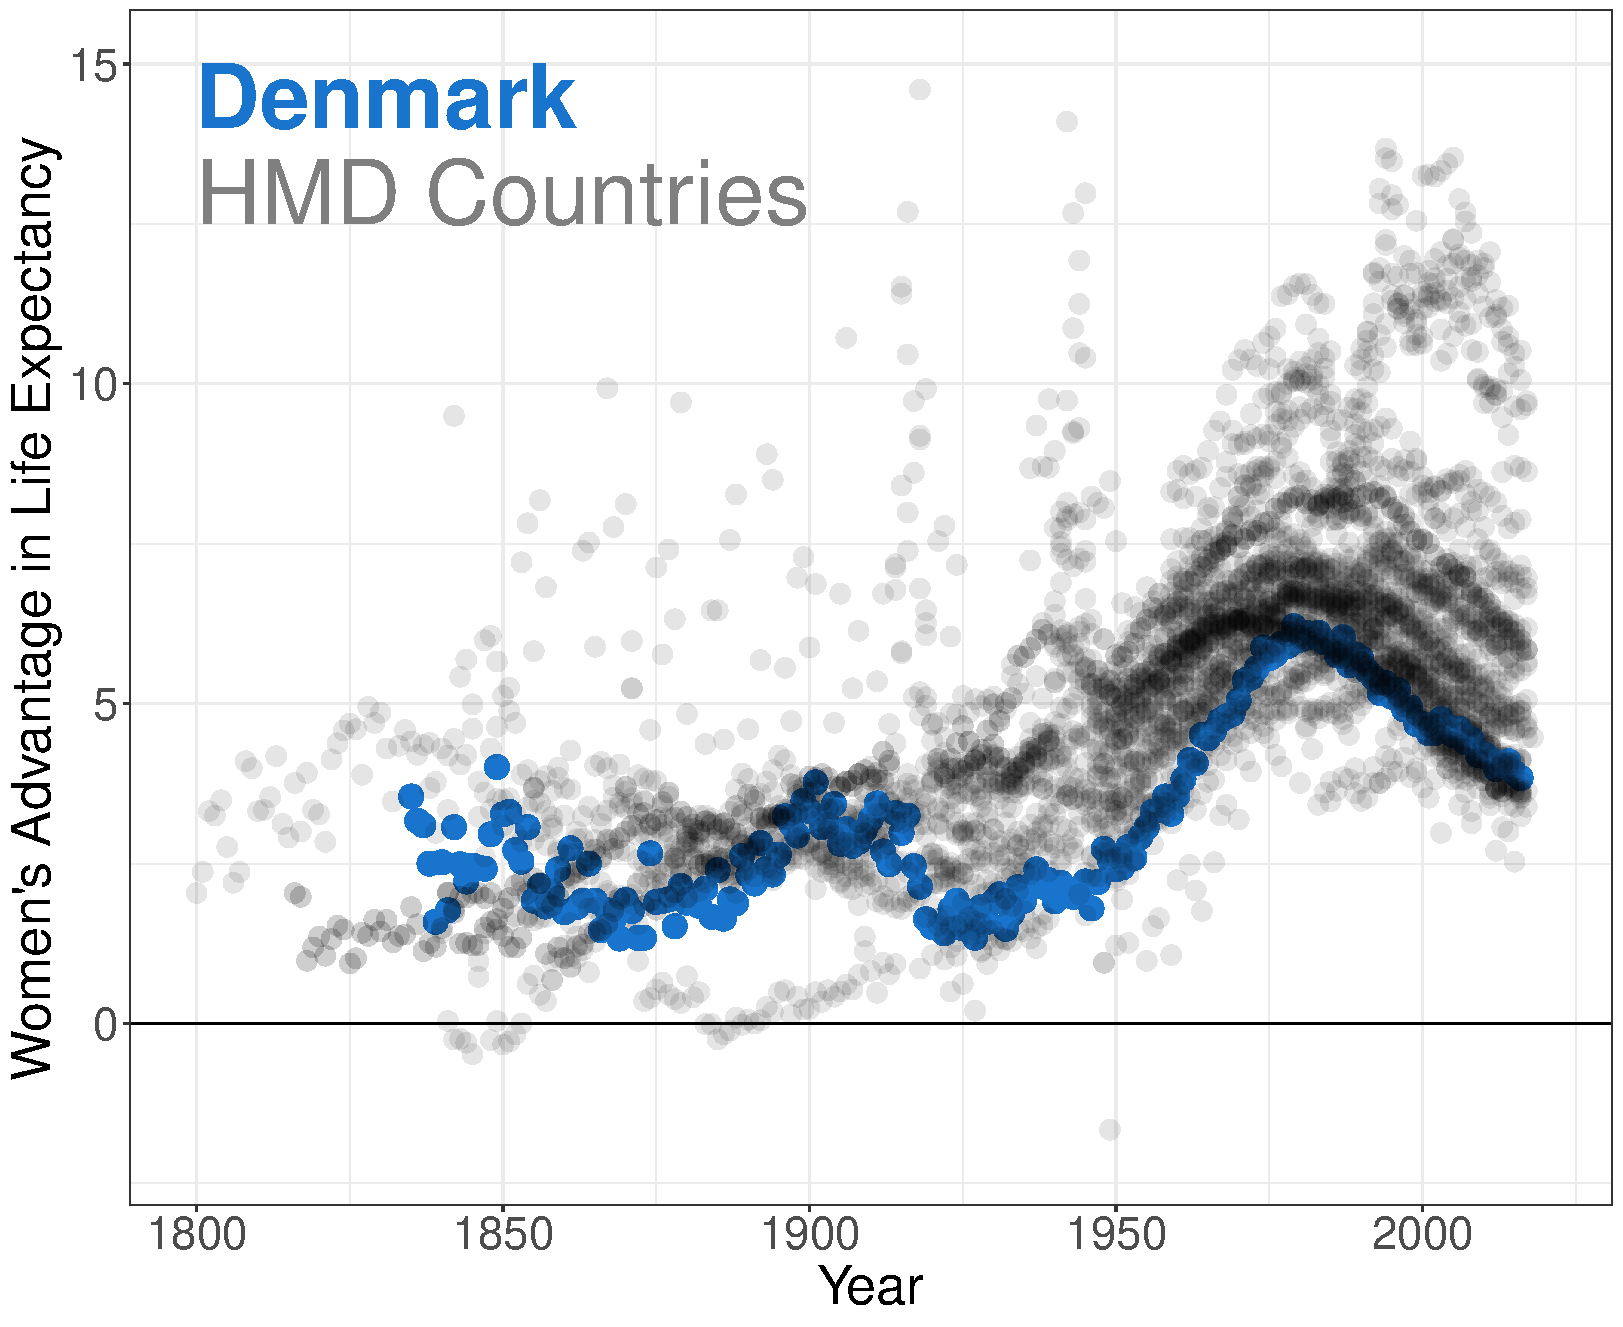
\includegraphics[scale=0.485]{Summary/PLOT/INTRODUCTION/PLOT_INTRO.pdf}
		\caption*{\textbf{Figure 1:} Women's absolute advantage in life expectancy at birth
									 in Denmark and all other HMD countries. 
									 \textit{Source: Own calculations based on HMD data.} }
		\label{ch1:fig1} 
	\end{figure}
	%--------------------%


%--------------------------------------------%
%--------------------------------------------%


\subsection{The Contribution of Behavior and Biology} 

% SIGNPOSTING %
In order to explain the rapid divergence and convergence of sex differences 
in life expectancy across developed countries throughout the 19th and 20th 
centuries, as well as cross-country differences in the timing of these trends, 
studies have drawn attention to behavioral aspects. In addition, studies 
have highlighted that mortality patterns at post-reproductive ages are an 
important part of the explanation for these patterns of divergence and 
convergence.\citep{thorslund2013,beltran2015}

% DIVERGENCE AND PEAK %
It has been shown that the widening sex gap in life expectancy throughout 
the 20th century was caused by the cohorts of men born in the late 19th 
century.\citep{beltran2015} Throughout the 20th century, men aged 50 to 70 
years old experienced slower mortality declines than women at these ages, 
which has been widely attributed to smoking.\citep{glei2007narrowing} 
During the 20th century, men had higher rates of smoking than women, and 
the prevalence of smoking among men increased at an earlier point in time.\citep{beltran2015}
Women picked up smoking, but with a delay of some decades.\citep{thun2012stages} 
During the peak of the gender gap in life expectancy, studies have estimated 
that differences in smoking accounted for up to 40\% of the gap in life 
expectancy in some countries.\citep{valkonen1997contribution} Alongside 
the lagged effect of smoking on mortality, men's higher propensity of 
hazardous drinking, poor nutrition, risk-taking behavior, higher levels 
of aggression and violence, and their reluctance to seek medical advice 
are assumed to have significantly contributed to sex differences in 
mortality.\citep{case2005sex,oksuzyan2008}

% CONVERGENCE %
Substantial changes in gender roles have reduced behavioral differences 
and, as a result, sex differences in life expectancy started to narrow 
since the 1970s.\citep{valkonen1997contribution} Support for this hypothesis 
comes from the observation that the prevalence of smoking increased 
among women born around the mid of the 20th century, while smoking rates had 
already started to drop among men of the same cohorts within most developed 
countries.\citep{lopez1994descriptive}

% CROSS COUNTRY %
Although behavioral factors are the largest drivers of cross-country 
differences in the magnitude of the gender gap when comparing Eastern 
and Western European countries, not all features of women's mortality 
advantage can be attributed to behavioral factors.\citep{luy2014impact}

% BIOLOGY %
One pattern that does not reflect behavioral causes is the fact that female infants 
have lower levels of mortality than male infants.\citep{drevenstedt2008rise} 
A consistent female advantage in mortality has also been found across historic 
populations who experienced extreme mortality conditions due to severe famines 
and epidemics -- an observation which has been interpreted as biologically-rooted.\citep{zarulli2018women} 
Quasi-natural experiments which have examined long-term trends in mortality among 
men and women in societies with strict behavioral rules and who have nearly 
identical lifestyles have also found a mortality advantage among women. Study 
populations included Mormons,\citep{lindahl2013male} Israeli Jews,\citep{staetsky2009unusually} 
and cloistered populations in Bavaria.\citep{luy2003causes,luy2009unnatural}

% BIOLOGY: GENETIC %
The two most plausible biological explanations for the female mortality advantage 
are differences in genes and endocrinology.\citep{hubbard2011frailty} Differences 
in the set of chromosomes are major genetic features that distinguish males and 
females. While males have one active X and one active Y chromosome in each cell, 
females have two X chromosomes, of which only one is active.\citep{christensen2001x} 
Studies have argued that the ability of the female organism to inactivate the 
disadvantageous X chromosome helps to prevent X-linked diseases and mutations, 
and weakens the effects of physiological stress on women compared to men.\citep{seifarth2012sex}

% BIOLOGY: HORMONES %
With regard to endocrinology, hormonal differences between the 
sexes, and in particular the strong sex-patterning of the steroid hormones 
estrogen, progesterone and testosterone, have been pointed out to have an impact 
on the female mortality advantage.\citep{regan2013gender} For example, higher 
estrogen levels in females were shown to have beneficial effects on serum lipid 
levels -- a major risk factor for the age at onset of cardiovascular diseases.\citep{eskes2007women} 
In addition, estrogen was shown to have immune-enhancing effects which may make 
females more resistant to certain infectious processes but more likely to suffer 
from autoimmune diseases.\citep{bouman2005sex}

% BIOLOGY: LIMITATIONS %
Despite all biological evidence, it needs to be taken into account that neither 
the exact impact of a single nor the sum of all biological factors can be 
estimated. In addition, not all species with sexual dimorphism show a 
general mortality advantage of females.\citep{austad2006women,austad2016sex}

% CONCLUSION %
Studies have increasingly argued that for human populations, gender is an 
important modifier of sex.\citep{rieker2005rethinking} For example, immune 
responses are strongly affected by social and environmental conditions, such 
as nutrition or the exposure to biologicals and chemicals.\citep{oertelt2012influence} 
To understand the origins of women's mortality advantage, a holistic, but 
the same time detailed perspective, is necessary that simultaneously explores 
mortality and health. \\


%--------------------------------------------%
%--------------------------------------------%


\subsection{The Paradox of Health and Survival}

Women's higher life expectancy at birth is the result of a universal 
mortality advantage. This advantage starts at infancy and can be found 
even at the highest ages, as absolute sex differences in mortality 
exponentially increase with age.\citep{carter1992modeling,gjonca2005,wisser2014sex} 
Women have lower rates of mortality with respect to most causes of death, 
as well as following most adverse life course events such as bereavement 
or job loss.\citep{martikainen1996excess,shor2012widowhood} However, 
women's mortality advantage does not translate into a universal health 
advantage -- a phenomenon known as the male-female health-survival 
paradox.\citep{oksuzyan2008,hubbard2011frailty}

Health is a multifaceted concept which incorporates various dimensions 
of physical, mental, and social well-being.\citep{who1946constitution} 
The recognized complexity of this concept has led to various approaches 
for measuring health and it's dimensions.\citep{mcdowell2006measuring} 
Although conclusions about the health status of individuals and populations 
depend on how health has been measured,\citep{patrick1989generic,ware1987standards} 
poor and declining health should be associated with lower levels of life 
expectancy.\citep{lee2000predictive,sasaki2007grip} However, this is not 
consistently the case when comparing men and women.

Empirical evidence for the existence of a male-female health-survival 
paradox has been reported widely over the past decades, and across a large 
number of countries.\citep{bambra2009gender,oksuzyan2010,nusselder2010gender,van2013gender} 
With respect to the physical dimensions of health, studies have shown 
that men have better physical performance and less functional limitations 
than same-aged women.\citep{nybo2001functional,oksuzyan2008,oksuzyan2010} 
Furthermore, men were shown to be less likely than women to report 
symptoms of depression, anxiety, and fear.\citep{mclean2011gender}

Another observation which has been interpreted as evidence for the paradox 
is that women, on average, use primary health care services more often 
than same aged men -- even when controlling for obstetrics-related 
treatments.\citep{wang2013men} However, it has remained unanswered whether 
higher levels of primary healthcare use among women are due to a lower 
threshold to seek medical treatment or a reflection of a true health 
disadvantage.\citep{hunt2011women,case2005sex} As it will be shown 
in the next section, lower levels of primary healthcare use among 
men are in contrast to their higher levels of hospital care use. 

A growing number of studies have begun to assess whether the health 
disadvantage of women is generalizable across all measures of health. 
These studies have shown that gender differences in health might be 
small or even reversed with regards to bio-markers and objective 
health measures.\citep{oksuzyan2014sex,oksuzyan2015} Even studies 
using survey data have shown that gender differentials in self-reported 
health substantially decrease or even flip when comparing men and 
women who have similar socioeconomic backgrounds, who engage 
in similar health behaviors, or when data for total populations 
are used.\citep{lynch2007use,crimmins2010gender,dahlin2013cross,
karampampa2013trends,jensen2014temporal,westergaard2019population}

Overall, it is  not yet fully understood whether gender differences in 
health reflect real differences or are likely to be explained by a number 
of distorting factors, such as gender-patterned survey participation rates 
or reporting styles.\citep{oksuzyan2009male,oksuzyan2019story} As it will 
be shown in the next section, patterns reported in existing studies using 
hospital admission data may question the generalizability of the health-survival 
paradox. \\ 


%-----------------------------------------------------------------------------------------%
%-----------------------------------------------------------------------------------------%


\section{Gender and Hospitalization}

\subsection{Hospitalization as a Health Indicator}

Routinely-collected hospital records are available for a variety of 
countries, such as the UK, Finland, Sweden, Norway, and Denmark. 
These data offer the potential to derive powerful indicators of 
health. In addition, hospital records may provide a unique framework 
for studying gender differences in mortality and health as these 
data cover information on medically diagnosed conditions and can 
often be linked with mortality data.

While contacts with primary healthcare services can be 
postponed or avoided, an admission to hospital is usually the 
consequence of a health deterioration that requires a needs-driven medical 
intervention.\citep{case2005sex,lynch2007use,westergaard2019population} 
Irrespective of whether an admission to hospital occurred due to a 
planned surgery or due to a sudden, life-threatening health shock, 
this contact with the healthcare system reflects a medical necessity. 
In both cases, a timely and medically more invasive intervention is 
required to prevent the worsening of health in the short or the long 
term, or even death.

A large number of previous studies have shown that the risk of hospitalization 
is strongly associated with a variety of well-established individual- 
and population-level health measures. With respect to individual-level 
health, poor self-rated health is a powerful predictor of an increased 
risk of hospital admission.\citep{kennedy2001repeated,desalvo2005predicting} 
A large number of studies have pointed out that certain behavioral 
factors are strongly associated with the risk of all-cause, as well 
as cause-specific hospital admissions. For example, smoking was shown 
to increase the risk of all-cause admissions, as well as the risk of 
hospitalization for neoplasms, through it's association with lung cancer.\citep{hanlon2000link} 
In addition, studies reported that hazardous drinking, being overweight, 
a poor diet, and a lack of physical activity are associated with an increased 
risk of all-cause and cause-specific hospital admissions.\citep{hanlon2007analysis,
smyth2015alcohol,reeves2014hospital,crowe2013risk,garcia2006regular,
syddall2016understanding}

In line with these observations at the individual level, studies have pointed 
out that the distribution of risk factors within populations is closely linked 
to population-level hospitalization patterns.\citep{hanlon2007analysis} 
For example, it has been argued that health behaviors and the health status 
of the underlying background population are closely associated with dimensions 
of population health, such as number of hospital admissions, bed days, 
cause-specific admission rates as well as rates of emergency admissions.\citep{busse2002use,
dixon2004hospital,luben2016predicting,syddall2016understanding,hu2018changes} 
Therefore, measures obtained from all-cause and cause-specific hospital 
admission data offer a pragmatic approach to monitor both population-level 
and individual-level health within a proxy framework. The potential of 
using routinely-collected, large-scale hospitalization records to study 
gender differences in mortality and health has not been fully realized.\\


%--------------------------------------------%
%--------------------------------------------%


\subsection{Gender Patterns in Admission and Mortality}

% INTRODUCTION: GENERAL STATEMENT %
The risk of hospitalization is strongly patterned by health 
conditions and increases with age as most non-communicable 
diseases become more prevalent.\citep{hanlon2000link,
hanlon2007analysis,hippisley2013predicting,campisi2013aging,
leening2014sex,rasmussen2018absolute} Generally, men and women 
at post-reproductive ages share a similar spectrum of diseases 
and disease co-occurrences when a life course perspective 
is taken.\citep{jensen2014temporal,westergaard2019population} 
However, when controlling for conditions and socio-demographic 
characteristics, the risk of all-cause and 
cause-specific admission to hospital consistently differs between 
men and women. For example, for most conditions, men are more 
likely to be admitted to hospital and get admitted at younger ages 
in comparison to women.\citep{hanlon2000link,case2005sex,
karampampa2013trends,luben2016predicting,westergaard2019population} 

% INTRO THE FIGURE %
\hyperref[ch1:fig2]{Figure 2} provides an overview of the average 
number of hospital days per person, across age, for Danish men 
and women using four different settings: (A) all patient types - 
all causes (B) all patient types - excluding obstetrics (C) excluding 
outpatients - all causes (D) excluding outpatients - excluding 
obstetrics.\footnote{Obstetrics-related admissions were defined 
as O.00-O.99 and Z.30-Z.39 according to the 10th Revision of the 
International Classification of Diseases (ICD-10)} 

% THE FIGURE %
As shown in \hyperref[ch1:fig2]{Figure 2}, irrespective of the 
specified setting, men spend more days in hospital than women 
during infancy and childhood. With the start of puberty, this 
pattern starts to change and women have higher levels of hospital 
bed days throughout the reproductive ages. At post-reproductive 
ages, the lines for men and women cross over in all settings and 
men, on average, spend more days in hospital than same-aged women. 
This male disadvantage in the risk of admission to hospital has 
also been reported for the oldest-old population in Denmark above 
the age of 90.\citep{engberg2009centenarians,oksuzyan2013changes} 
When comparing the panels in the left column with the panels in 
the right column, it becomes evident that the higher level of 
hospital bed days among women across reproductive ages is directly 
linked with obstetrics-related admissions.\\


	%------------------%
	\begin{figure}[H]
		\centering
		% PLUG IN REVISED FIGURE %
		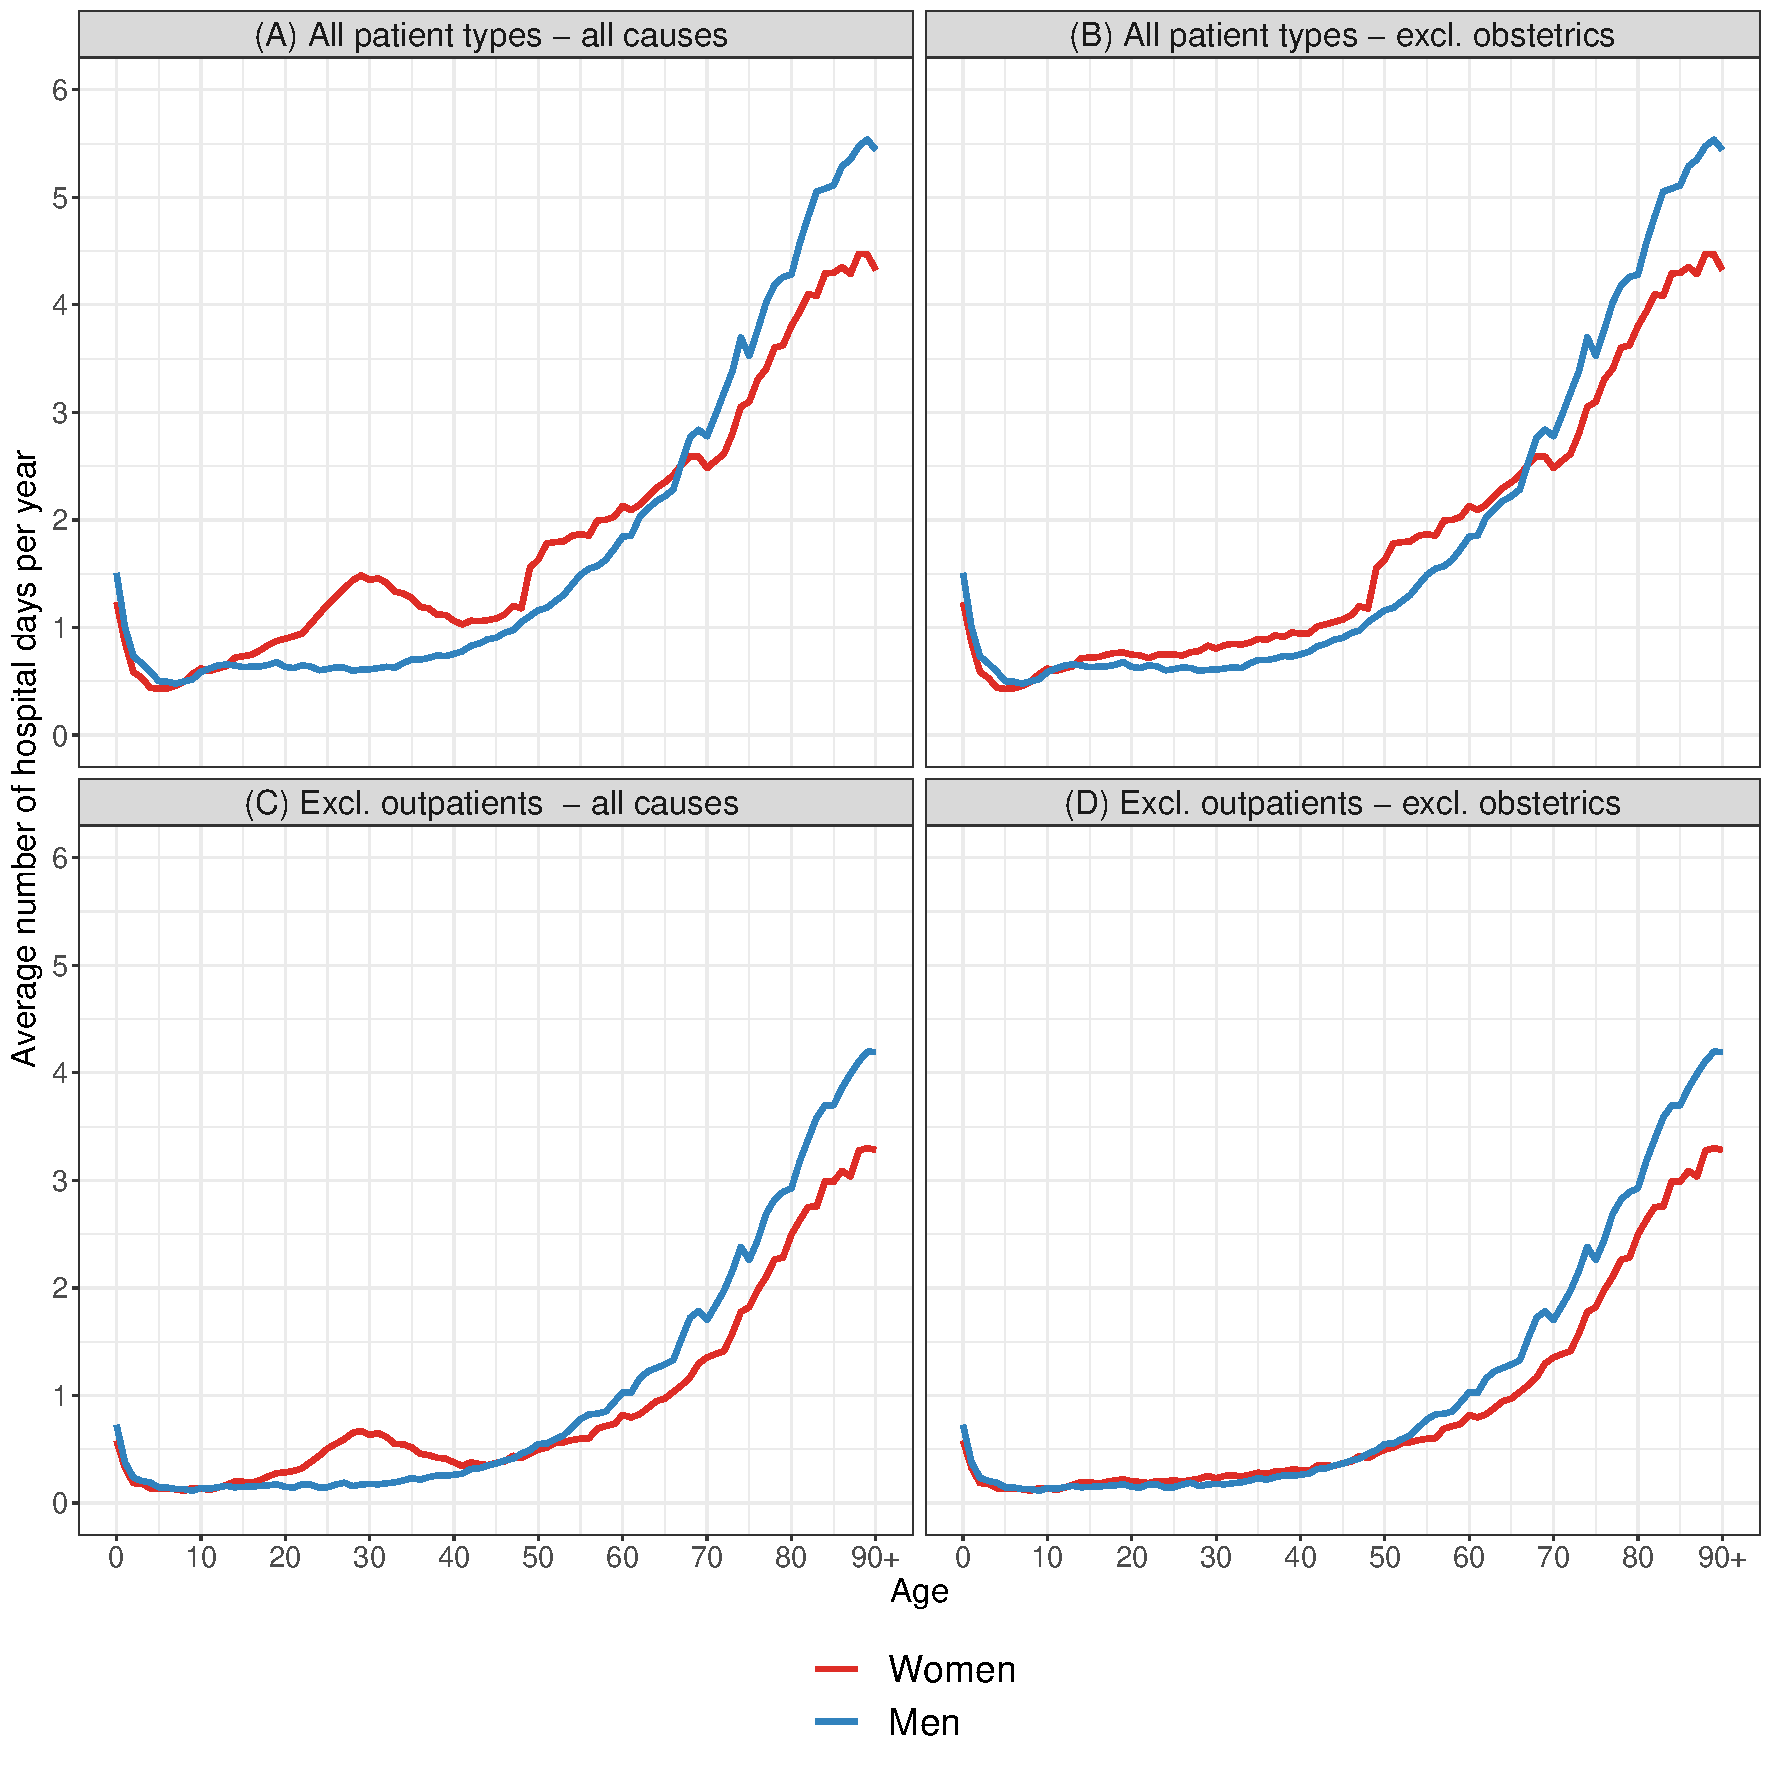
\includegraphics[scale=0.425]{Summary/PLOT/HEALTHCARE_ANALYSIS/HOSP_Patterns.pdf}
		\caption*{\textbf{Figure 2:}    Sex differences in hospital care use in Denmark, 2014.
										\textit{Source: Own calculations based on register data 
										for the total Danish population.} 
										}
	\label{ch1:fig2} 	
	\end{figure}
	%--------------------%


% DIFFERENCES IN CAUSES OF ADMISSION %
A cause-specific perspective is needed to further understand 
why men have higher levels of hospital care use at post-reproductive 
ages in comparison to women. Women have a higher risk of admission 
to hospital for a number of less life-threatening conditions, 
such as diseases of the eye or musculoskeletal disorders,\citep{simmonds2014understanding,
westergaard2019population,rollman2001sex} as well as conditions 
which can be treated in outpatient settings.\citep{jensen2014temporal}  
In contrast, men at post-reproductive ages have a higher risk of 
being admitted to hospital for the majority of other diseases, 
including cardiovascular diseases, neoplasms, respiratory diseases, 
and diseases of the digestive system.\citep{simmonds2014understanding,
westergaard2019population} Even when controlling for age, health 
behaviors, and co-morbidity, men have a higher risk of being admitted 
to hospital and to die following admission than women with the same 
conditions.\citep{case2005sex} 

% MORTALITY FOLLOWING ADMISSION %
Women experience lower mortality following most causes of admission to 
hospital than same-aged men. This is the case for most neoplasms,\citep{cook2011,
jung2012female,radkiewicz2017sex} chronic obstructive pulmonary disease 
(COPD),\citep{de2009sex,gonzalez2011gender} Pneumonia,\citep{kaplan2002hospitalized,
reade2009differences} or hip fractures.\citep{kannegaard2010excess,katsoulis2017excess} 
In contrast, findings for myocardial infarction (MI) and stroke were 
ambiguous. Some studies report no gender differences or even a mortality 
disadvantage among women following an admission for stroke\citep{appelros2009sex,
appelros2010review,kim2010gender,andersen2011predictors} and MI\citep{simon2006impact,
nielsen2014sex}. However, women tend to be significantly older than 
their male counterparts at disease onset, and age-specific incidence 
rates for these causes are usually higher in men than in women.\citep{kim2010gender,
appelros2009sex}

% MORTALITY FOLLOWING ADMISSION %
Previous studies have provided valuable insights into gender 
differences in the risk of hospitalization and mortality 
following admissions. However, important gender-patterns 
surrounding hospital admissions are not yet fully understood -- 
for example whether the magnitude of gender differentials in 
mortality changes following an admission to hospital when 
compared with the differential in the general population. 
The next section provides an overview of specific research 
gaps, which have been addressed in the thesis. \\

%--------------------------------------------%
%--------------------------------------------%


\subsection{Research Gaps}

% LINK TO PAPER 1 %
The mortality advantage of women is well explored in general populations 
and following most causes of admission to hospital. It is also well-established 
that men are more likely to die following hospitalization, suggesting that 
the implications of deteriorating health are stronger in men than in 
women.\citep{hanlon2000link,case2005sex,hubbard2011frailty} However, it 
is not yet known whether the magnitude of women's  mortality advantage 
increases or decreases following all-cause and cause-specific hospital 
admissions when compared with women's mortality advantage in the general 
population. 

% LINK TO PAPER 2 %
One important observation among previous studies is that women, on average, 
engage with primary healthcare services more often in comparison with 
same-aged men.\citep{case2005sex,juel2008men,oksuzyan2008,wang2013men,
banks2013men,wang2014gender} On the one hand side, these studies interpreted 
this pattern as an indicator of women's poorer health. On the other 
hand side, these studies have argued that this may be the reason why 
women are less likely to be admitted to hospital and have lower levels 
of mortality. Therefore it remains unclear whether women's 
higher levels of primary healthcare use are due to a potential health 
disadvantage or whether they reflect a lower threshold to seek medical 
advice.\citep{hunt2011women} Looking at changes in treatment-seeking 
behavior surrounding hospital admissions may provide valuable insights 
into this debate.

% LINK TO PAPER 3 %
Research has shown that increases in the age at first admission to 
hospital for men and women at post-reproductive ages have kept pace 
with increases in average life expectancy.\citep{karampampa2013trends} 
This was considered as evidence of morbidity compression. Studies 
of morbidity compression typically measure progress in health and 
life expectancy in terms of averages.\citep{colvez1983potential,
robine1999health,beltran2015past,salomon2012healthy,crimmins2016trends} 
Despite the rapidly improving quantity, quality and availability 
of health data, for example provided by the Global Burden of Disease 
Study,\citep{global2019} variation in age at morbidity onset has largely been overlooked. 
One part of the explanation is that it is challenging to estimate 
long-term trends in morbidity incidence reliably for total 
populations.\citep{modig2013age,modig2017estimating,modig2019temporal}
Routinely-collected hospital admission data, collected for an entire 
population and consistently over a long period of time, provide a unique 
framework for identifying changes in the first incidence of a medically 
diagnosed condition.\citep{lynch2007use,karampampa2013trends,westergaard2019population,
jensen2014temporal} From these data, measures of variation in 
age at morbidity onset can be estimated. This is particularly 
important for understanding the extend of gender differences 
in health beyond average measures. The amount of variation indicates the level 
of uncertainty individuals can expect in the timing of health deterioration.\citep{van2018case}
At the population level, welfare states will have to adapt to the heterogeneous 
needs of aging populations.\citep{van2014lifespan,sasson2016trends,van2018case} 

% LINK TO PAPER 4 %
The demographic structure of the population has important implications 
for the provision of healthcare, including hospital settings.\citep{christensen2009ageing,
beard2015towards} On average, older individuals have higher levels 
of hospital care use than younger individuals.\citep{pallin2014us} 
Furthermore, the incidence of most non-communicable diseases, such 
as cardiovascular diseases,\citep{leening2014sex} cancers,\citep{campisi2013aging} 
and dementia\citep{rasmussen2018absolute} are strongly patterned by 
sex and age. Therefore, one important consequence of population 
aging is that the demographic composition of patients in need of 
hospital care is likely to change. An adequate supply and mix 
of well-trained health workers will be necessary to meet the needs 
of future patients.\citep{darzi2016global} In addition, forecasting 
the structure of future hospital patients with respect to both, age 
and sex, is particularly important for the education of the future 
medical workforce.\citep{meiboom2015medical,samra2015medical,samra2017factors} 
Part of the reason is that the medical workforce in training, including 
medical doctors and student nurses, tends to have negative attitudes 
towards older patients -- factors which were shown to have a significant 
impact on career choices as well as the quality of care and treatment.\citep{hughes2008medical,
samra2015medical,kusumastuti2017contact,fisher2018pejorative} \\


%-----------------------------------------------------------------------------------------%
%-----------------------------------------------------------------------------------------%


\section{Denmark -- The Context of the Thesis}

% GENERAL INTRO %
Denmark, the geographical focus of the thesis, has similar gender 
patterns in mortality and health to those observed in most developed 
countries.\citep{human2005university,bronnum2005health,van2013gender,
jeune2008trends} In addition, Denmark is an example country which 
clearly illustrates that the magnitude of gender differences in 
mortality is affected by modifiable factors.

% LE TRENDS BRIEFLY %
In Denmark, the difference in life expectancy between men and women 
was 3.6 years in 1835, and this gap reached a peak in 1979 at 6.2 
years.\citep{human2005university} In between these years, and as 
previously illustrated in \hyperref[ch1:fig1]{Figure 1}, the magnitude 
of gender differentials in life expectancy has been relatively low in 
Denmark when compared to other HMD countries. In 2016, Danish women 
outlived Danish men by 3.8 years. 

% INTRODUCING UNIQUE FRAMEWORK
Denmark provides a unique framework for studying gender differences 
in mortality, as improvements in life expectancy among Danish women 
stagnated between the 1970s and 1990s.\citep{jacobsen2002,bronnum2005health,
jeune2008trends,aburto2018potential} Studies have identified that this 
stagnation was driven by the cohorts of Danish women born between the 
two world wars and is closely related to the  the emergence of smoking 
in these cohorts.\citep{jacobsen2004women,lindahl2016did}

% COHORT PHENOMENON %
More specifically, Danish women born between 1915 and 1945 had a 
high prevalence of smoking throughout their entire lives, resulting 
in high death rates from smoking-attributable diseases relative to 
most other European countries.\citep{jacobsen2006} The effect of smoking 
on population-level mortality is not immediate, and subject to a lag 
effect.\citep{lopez1994descriptive} Therefore, it took multiple decades 
for this pattern to become visible in Denmark. As these cohorts of Danish 
women are now dying out, the phenomenon of stagnating life expectancy is 
diminishing.\citep{jacobsen2016} Within the past two decades, the life 
expectancy of women in Denmark has increased faster than for women in 
Sweden and Norway.\citep{jacobsen2016} Nevertheless, the life expectancy 
of Danish women is still lower than in most Western European countries 
today.\citep{human2005university,human2005university} 

% DK DATA AVAILABILITYY
In pragmatic terms, Danish register data provide a unique tool for 
studying differentials in mortality and health.\citep{frank2000entire,
schmidt2014,thygesen2014entire} These data have a similar structure, 
validity, and coverage as the registers in the other Nordic Countries.\citep{olsen2010high,
thygesen2014entire,maret2017nordic} The data utilized in the thesis 
include information on contacts with different sectors of the Danish 
healthcare system and basic demographic information covering the 
entire population alive and residing in Denmark.

% DK HEALTH CARE %
A universal healthcare system is a particular feature of the Danish 
welfare state. This system is the outcome of a long path of political 
decision-making, which traditionally focused on public welfare 
services in order to reduce socioeconomic inequalities.\citep{vrangbaek2005health}
In Denmark, healthcare is financed through taxes and access to healthcare 
services is free for all residents.\citep{juul2012denmark,pedersen2012general} 
This means that this healthcare system should reduce systematic exclusions 
and hurdles in accessing healthcare services among men and women of 
post-reproductive ages. Within this framework, general practitioners 
(GPs) have an essential gate-keeping role regarding the use of hospital 
care.\citep{sahl2011danish,juul2012denmark,pedersen2012general} Therefore, 
an admission to hospital in Denmark represents a needs-driven interaction 
with the healthcare system. \\


%-----------------------------------------------------------------------------------------%
%-----------------------------------------------------------------------------------------%


\section{Aims and Objectives}

The thesis aims to study gender differences in mortality and health using 
hospitalization records for the Danish population at post-reproductive ages. 
The following research objectives were chosen to achieve this aim:

\begin{enumerate}
	\item	Measure changes in the magnitude of women's mortality advantage 
			following the deterioration of health (Paper 1).
	\item	Compare gender differences in treatment-seeking behavior 
			before and after a major health shock (Paper 2).
	\item	Quantify the mean age, and variation in the mean age, at 
			disease onset among men and women (Paper 3).
	\item	Forecast changes in the demographic structure of hospital 
			patients due to population aging (Paper 4).\\
\end{enumerate}


%-----------------------------------------------------------------------------------------%
%-----------------------------------------------------------------------------------------%


\section{Methods and Materials}

\subsection{Data}

% SIGNPOSTING %
A major similarity among all five Nordic Countries -- Norway, Iceland, 
Finland, Sweden, and Denmark -- is the structure of their population-based 
register systems.\citep{maret2017nordic} Despite the relatively small 
population sizes of these countries, their registers can ensure large 
sample sizes as the total population is covered.\citep{olsen2010high,
maret2017nordic} Since the introduction of the personal identification 
numbers in the 1960s, individuals in the Nordic Countries can be 
followed throughout different registers. This unique structure enables 
complex life course perspectives in epidemiological studies.\citep{thygesen2014entire}

% INTRO: DENMARK %
In the thesis, three different Danish registers were used: the Central 
Population Register (CPR), The National Patient Register (NPR), and 
The National Health Service Register (NHSR). \hyperref[ch1:fig3]{Figure 3} 
illustrates the different time periods for which data were available from 
each register.

% DESCRIBTION %
Although these registers were created primarily for administrative 
reasons, they can be accessed for research purposes.\citep{andersen1999,
schmidt2014,thygesen2014entire} A 5\% sample was used for the first paper. 
In all subsequent papers, the data covered the total Danish population. 
The following section provides an overview of the three registers. A 
more detailed and tailored description of how these data were handled 
is provided in each paper. The strengths and limitations of these data 
are critically evaluated in the discussion section at the end of this 
chapter. \\


	%------------------%
	\begin{figure}[H]
		\centering
		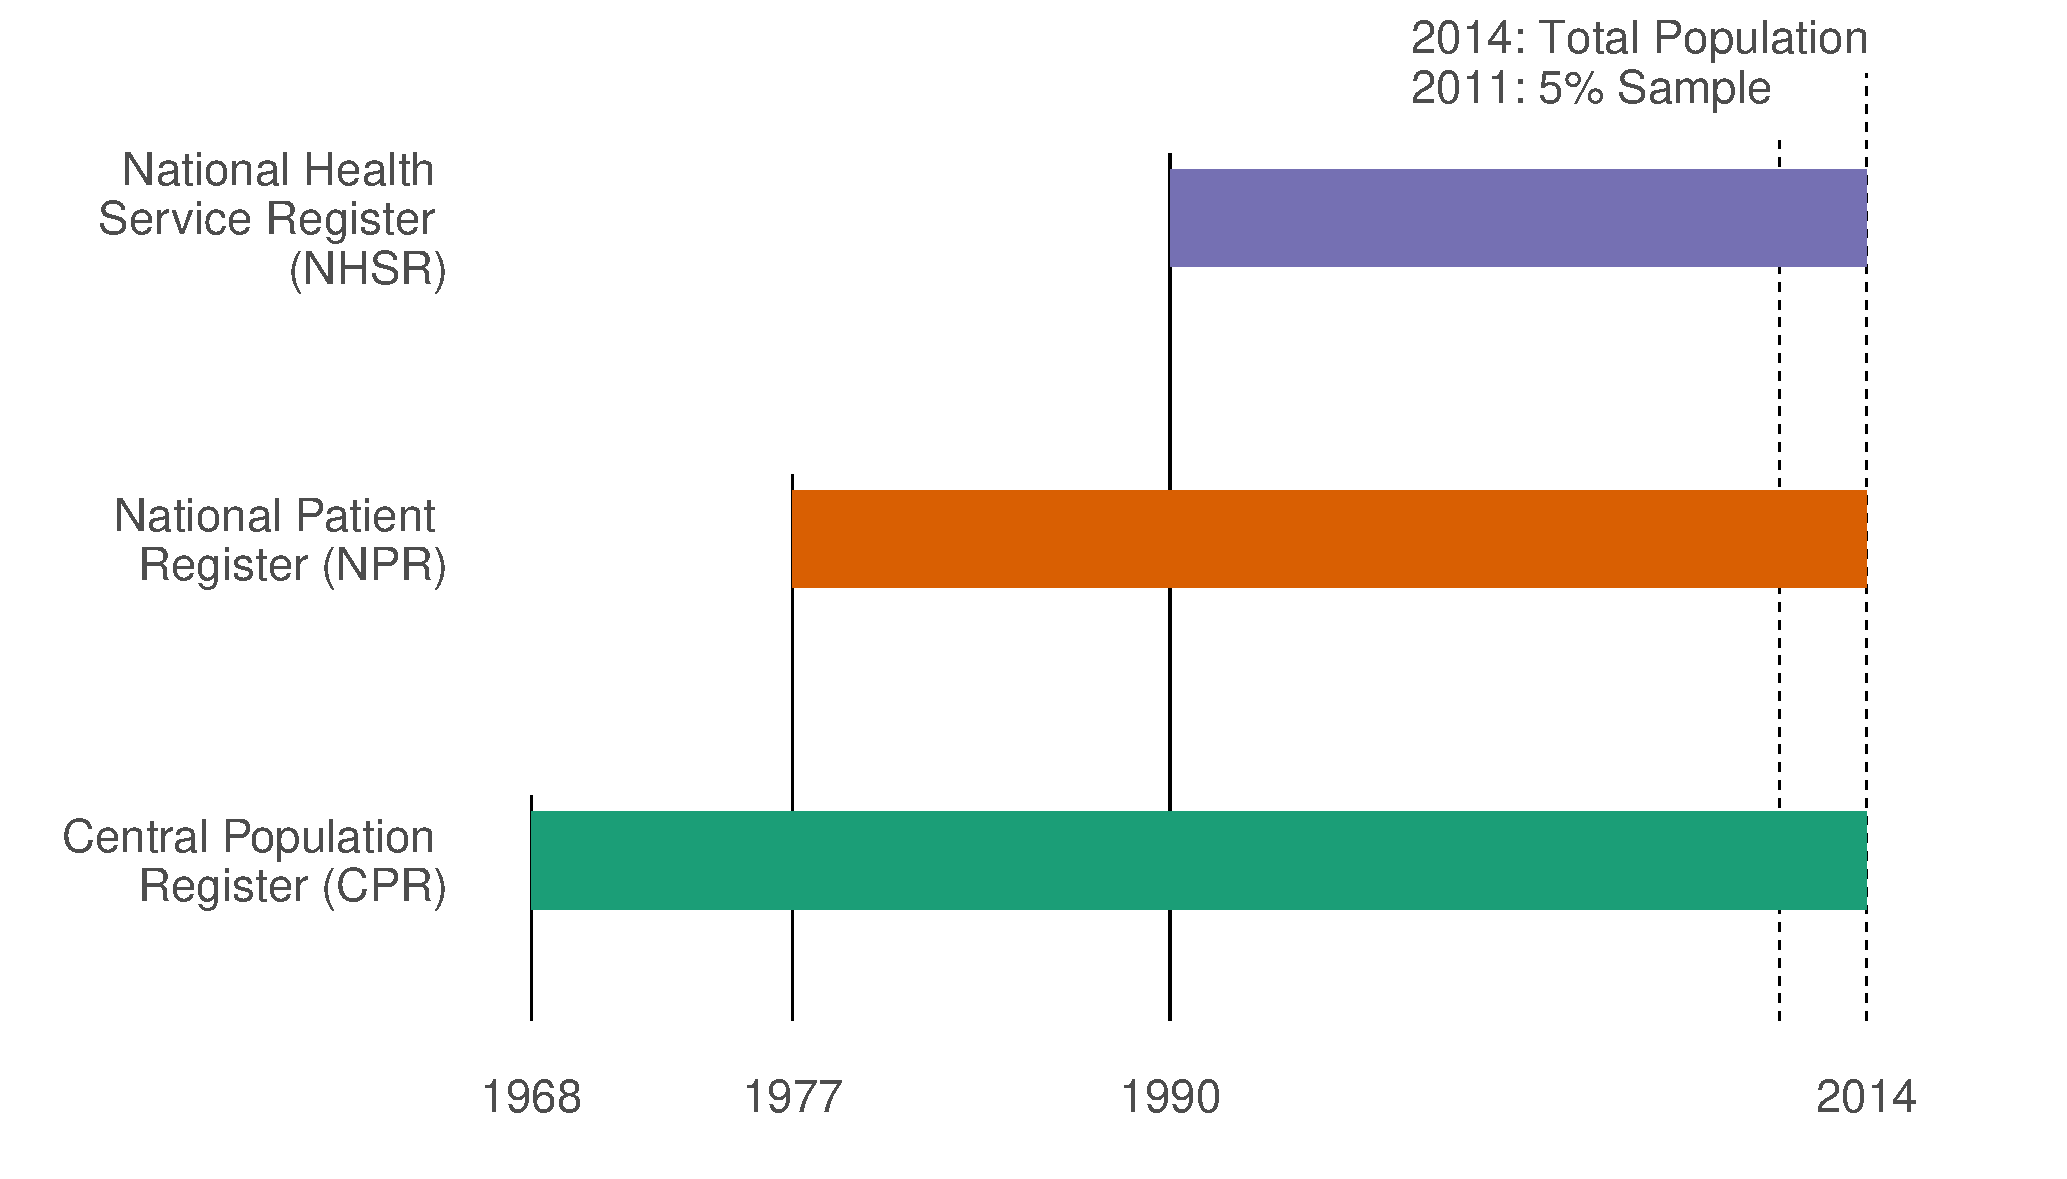
\includegraphics[scale=0.425]{Summary/PLOT/DATA/PLOT_DATA.pdf}
		\caption*{\textbf{Figure 3:} Overview of the utilized data sources.}
	\label{ch1:fig3} 
	\end{figure}
	%--------------------%
	
	
\subsubsection*{Central Population Register (CPR)}
In 1875, a register on causes of death was established in Denmark.\citep{thygesen2011} 
Since 1924, information on all Danish residents have been collected and 
continuously updated within municipal registers for administrative and 
planning purposes.\citep{malig1996civil} In 1968, this system was replaced 
by a centralized civil registration system.\citep{pedersen2006} Since then, 
demographic information on each resident's vital status, sex, and date of 
birth have been electronically recorded in the CPR. A unique personal 
identification number (CPR-Number) has been assigned to all individuals 
residing in Denmark.\citep{pedersen2011} Information in other Danish 
registries are collected and saved using the CPR-Number. This enables 
deterministic linkage of different population-based registers.\\

%--------------------------------------------%

\subsubsection*{National Patient Register (NPR)}
Data on hospital admissions were accessed via the NPR. The NPR was established 
in 1977 and covers administrative and medical information on hospital care 
provided in Danish hospitals.\citep{schmidt2015danish} While inpatient 
treatments have been recorded since 1977, outpatient treatments, information 
from psychiatric wards, and emergency admissions have only been included 
since 1995.\citep{lynge2011} Despite this increase of covered information as 
well as the introduction of new classification systems, for example the change 
from ICD-8 to ICD-10 in 1994,\citep{munk1999implementation} individuals can 
be followed consistently over the entire range of time. This makes the 
hospitalization register a high-quality source of data for epidemiological 
research.\citep{lynge2011}\\

%--------------------------------------------%

\subsubsection*{National Health Service Register (NHSR)}
Data on the primary healthcare use of the Danish population is recorded 
in the National Health Service Register (NHSR). The NHSR was established 
in 1990 and contains data from health contractors in primary healthcare 
settings on the service provided and the citizen who received treatment.\citep{thygesen2011} 
Treatment of children under age 16 was reported under the CPR-Number of 
one parent until the end of 1995.\citep{sahl2011danish} To avoid potential 
bias emerging from this feature, papers in the thesis which utilized data 
from the NHSR, excluded information prior 1996. A summary of the data 
sources used for each paper is given in \hyperref[ch1:tab1]{Table 1}.\\


	%-------------------------------------------------------%
	% SUMMARY TABLE ON UTILIZED REGISTERS AND STUDY PERIODS %
	\begin{table}[htbp]
  		\centering
 		 \caption*{\textbf{Table 1:}   Overview of utilized data sources, sample sizes, and study periods 
  									   covered in the papers of the thesis.}
    	\begin{tabular}{lccc}
    	\toprule
    	\multicolumn{1}{c}{\textbf{Paper}} & \textbf{Sample Size} & \textbf{Register} & \textbf{Period} \\
    	\midrule
    	1: Mortality 			& 5\% Sample	 & CPR, NPR 		& 1977 -- 2011 \\
    	2: Treatment-Seeking	& Total Pop. 	 & CPR, NPR, NHSR 	& 1992 -- 2014 \\
    	3: Variation 			& Total Pop. 	 & CPR, NPR 		& 1977 -- 2014 \\
    	4: Forecasting		    & Total Pop. 	 & CPR, NPR, NHSR 	& 2014 \\
    	\bottomrule
    	\bottomrule
   		\end{tabular}%
   	\vspace{0.15in}
   	\label{ch1:tab1}
	\end{table}%
	%-------------------------------------------------------%


%----------------------------------------------------------------%
%----------------------------------------------------------------%


\subsection{Methods}

The thesis focuses on studying health and mortality using hospital 
admission data. As the population of post-reproductive ages was focused, 
a potential sex bias, caused by admissions for reproduction and 
child birth, is substantially reduced. However, when necessary, 
the impact of obstetrics-related admissions was controlled for.

Particularly at post-reproductive ages, contacts with the healthcare 
system, including hospitals, are frequent events. In all papers of 
the thesis, sample sizes were large -- even when stratifying study 
populations by age, sex, and cause of admission. The properties of 
the register data provide a unique opportunity to utilize both 
individual-level and aggregate-level methods, as well as to incorporate 
cross-sectional and longitudinal 
perspectives. 

This section provides a brief description of the methods applied in each 
paper, and a justification for why they were used. A summary of the methods 
used in each paper is provided in \hyperref[ch1:tab2]{Table 2}. Details 
of the modeling processes and results of sensitivity analyses are 
presented within each paper. \\


	%-------------------------------------------------------%
	\begin{table}[H]
    	\centering
 		\caption*{\textbf{Table 2:}  	Overview of methods and perspectives 
 										in the papers of the thesis.}
    	\begin{tabular}{lcl}
    	\toprule
   		\multicolumn{1}{c}{\textbf{Paper}} & \textbf{Perspective} & 
   		\multicolumn{1}{c}{\textbf{Utilized Methodology}} \\
    	\midrule
    	1: Mortality  & Ind. Level & GAMs, Splines\\
    	2: Treatment-Seeking & Ind. Level & Hurdle Models, Splines\\
    	3: Variation & Pop. Level & Life Tables and Variation Measures\\
    	4: Forecasting & Pop. Level & Deterministic Forecasting\\
    	\bottomrule
    	\bottomrule
   		\end{tabular}%
 	\vspace{0.15in}
 	\label{ch1:tab2}
	\end{table}%
	%-------------------------------------------------------%


\subsubsection*{Generalized Additive Models (GAMs)}

The first paper explored levels of mortality among men and women 
following the first all-cause and cause-specific admission to hospital 
after age 50. Levels of mortality, and in particular the absolute sex 
differences in mortality, were compared with the levels observed in two 
matched reference populations: a general and a temporarily non-hospitalized 
population. Matching based on sex and day of birth was used to ensure 
that populations share an identical demographic structure.\citep{rothman2008modern} 
For hospitalized individuals, the survival time started on the first day 
of hospitalization and ended either due to death within 1 year following 
admission or censoring. The survival time of matched individuals in each 
reference population started the day the corresponding case was admitted 
to hospital and ended either due to death within 1 year or censoring. GAMs 
with a binary link\citep{hastie1995generalized} and penalized b-splines 
('p-splines')\citep{eilers1996flexible} were used to estimate the levels 
of mortality. Mortality was estimated separately for the men and and 
the women of each population.

In contrast to generalized linear models (GLMs), the linear predictor 
in a GAM is replaced by a sum of smoothing functions.\citep{hastie1986generalized,
hastie1995generalized} This non-parametric approach allowed the risk of 
mortality to follow non-linear trajectories over age as the estimated 
mortality trajectories are not predefined by the functional form of a 
GLM.\\

%--------------------------------------------%

\subsubsection*{Hurdle Models}

The second paper examined whether patterns of treatment-seeking behavior 
surrounding a major health shock differed between men and women. For this 
paper, a hurdle model was used.\citep{min2005random,rose2006use,hu2011zero} 
The application of a hurdle model matched the full potential of the data as 
individuals who did not consult with primary healthcare services could be 
identified. This approach allowed for a distinction between two stochastic 
processes: the risk of being a non-user of primary healthcare, and the rate 
of healthcare use among those who engage with primary healthcare.\citep{gerdtham1997equity} 
This distinction is important as there might be no difference between men and 
women who did engage with healthcare services -- a feature an aggregate-level 
approach would have overlooked. Applying a hurdle model enabled the research 
question to be answered from a longitudinal perspective, as changes in the 
magnitude of gender differences in primary healthcare use following hospitalization 
could be studied.

The hurdle model estimated the levels of non-use of primary healthcare 
as well as the number of contacts with primary healthcare among users 
surrounding the first inpatient admission to hospital after age 60 for 
four conditions: stroke, MI, COPD, and gastrointestinal cancers (GIC). Hurdle 
models combine a logistic model for the probability of zero-counts with 
a regression model for the positive counts.\citep{min2005random} In order 
to account for repeated observations, hurdle models allow for the incorporation 
of individual random effects.\citep{min2005random} \\

%--------------------------------------------%

\subsubsection*{Life Tables and Life Span Variation Measures}

In the third paper, time-to-admission life spans were estimated in order 
to quantify the mean age at morbidity onset and variation in the mean age. 
For each year, all individuals aged 60+ who were at risk of experiencing 
a first admission to hospital, as well as those who were actually admitted, 
were identified. A 7-year washout period was applied in order to ensure 
that the first admission to hospital was not a re-admission or a follow-up 
treatment. Time-to-admission life spans started on the 60th birthday and 
ended the day of the first inpatient admission to hospital for all-causes. 
This setting enabled the estimation of age-specific risks of first admission 
for men and women for each year of the study period. Age-specific risks were 
then used to construct period life tables and calculate lifespan variation 
measures for each year, and for men and women separately.\citep{preston2000demography} 
Variation in the mean age was measured using the coefficient of variation -- 
a relative measure, which accounts for changes in the mean. 95\% confidence 
intervals (CI) for life table parameters were estimated using the approach 
provided by Chiang (1984).\citep{chiang1984lifetable} \\

%--------------------------------------------%

\subsubsection*{Deterministic Baseline Forecasting}

In the fourth paper, a deterministic baseline forecast was used to examine 
how the current demographic structure of hospital care use may change due 
to population aging.\citep{ganguly2016using,bohk2018forecast} In a first 
step, the total Danish population was followed up for inpatient and emergency 
admissions recorded in Danish hospitals in 2014. This enabled the estimation 
of the baseline year levels: the age- and sex-specific patterns of hospital 
care use in 2014. The baseline-year levels were estimated by dividing the 
number of hospital days by the corresponding population at risk. The baseline 
levels were kept constant throughout the entire projection period and 
multiplied with the most recent population estimates provided by Statistics 
Denmark.\citep{denstat2018frdk218,denstat2018projection} This enabled a 
deterministic quantification of hospital care use on the national level 
up to the year 2050. As patterns observed in the baseline year 2014 were 
kept constant throughout the entire study period, changes in the age- 
and sex-specific patterns of hospital days were driven entirely by changes 
in the demographic structure of the Danish population, and in particular 
population aging.\\


%-----------------------------------------------------------------------------------------%
%-----------------------------------------------------------------------------------------%


\section{Results and Discussion}

\subsection{Main Findings and Contribution to Existing Knowledge}

\subsubsection*{Sex Differences in Mortality Following Hospitalization}

% RESULTS %
The first paper estimated the magnitude of male excess mortality in 
the 1-year risk of dying following a deterioration of health, measured 
as the first all-cause and cause-specific hospital admission after 
age 50. A comparison was made with the corresponding male excess 
mortality observed in a matched general and temporary non-hospitalized 
population. In all populations, women had consistently lower mortality 
than men. Furthermore, absolute sex differences in mortality were 
always highest in the hospitalized population, followed by the general 
population, and the temporary non-hospitalized population. This gradient 
was consistent across all-cause as well as selected cause-specific 
hospital admissions.

% CONTRIBUTION %
Findings of the first paper indicate that part of women's mortality 
advantage after age 50 can be attributed to their lower risk of dying 
following health deterioration. While it is likely that 
behavioral and biological aspects have contributed to the mortality 
differentials following hospitalization, for example differences 
in treatment-seeking behavior and immune response,\citep{case2005sex,
juel2008men,oertelt2012influence,wang2014gender} the exact causes for 
the observed patterns could not be disentangled. Nevertheless, findings 
of the first paper provide valuable insights into the underlying mechanisms 
of women's mortality advantage at post-reproductive ages: Women have lower 
mortality after the onset of health deterioration while likely remaining 
alive in bad health. The finding that women had lower mortality 
following all studied causes of admission indicates that sex differences 
in the distribution of the causes of admission do not explain sex differences 
in mortality after all-cause hospital admission.\\

%--------------------------------------------%

% PAPER 2 - ALL DONE  %
\subsubsection*{Gender-Specific Changes in Treatment-Seeking Around Admission}

% FINDINGS %
The second paper examined a potential factor contributing to women's 
mortality advantage following hospital admission: their higher propensity 
to seek medical advice before health deterioration.\citep{o2005s,juel2008men,
oksuzyan2008,banks2013men} In the paper, gender patterns in treatment-seeking 
around the first inpatient hospitalization after age 60 were studied. 
Using a hurdle model, levels of primary healthcare use and levels of 
non-use before and after hospitalization for stroke, MI, COPD, and 
GIC were estimated. Before hospitalization, 
men were substantially more likely to be non-users and had fewer 
contacts with primary healthcare given that they were users. The 
use of primary healthcare services increased substantially among 
men and women following hospitalization. However, levels of non-use 
dropped more sharply among men and increases in the level of healthcare 
use were more pronounced among men users. Although the magnitude 
of absolute gender differences in primary healthcare use decreased 
sharply following hospitalization, differences between men and women 
never fully vanished.

% CONTRIBUTION %
The second paper contributed to the question of whether women utilize 
primary healthcare services more often -- and if yes, why.\citep{case2005sex,
juel2008men,hunt2011women,wang2013men,wang2014gender} Studying these questions 
within a longitudinal, individual-level framework is a valuable 
contribution as the majority of quantitative studies have utilized 
cross-sectional data on the aggregate level.\citep{juel2008men,banks2013men,
wang2013men} In addition, a major contribution is that the application of 
hurdle models allowed two features to be distinguished: non-use and levels 
of use among the user group. This is important as gender differences in 
mean levels might be due to differences in the share of users and non-users 
among men and women. The findings of the paper show that women's higher 
levels of primary health care use are likely to be due to both a lower 
threshold for treatment-seeking and a health disadvantage at older ages, 
emerging from women's lower mortality following hospitalization. It is 
known that repeatedly missing appointments is associated with an increased 
risk of mortality.\citep{McQueenie2019} However, future research should 
examine the association between gender-patterned treatment-seeking behavior 
and gender-patterned mortality following hospital admissions.\\

%--------------------------------------------%

% PAPER 3 - ALL DONE %
\subsubsection*{Inequalities in Mean Age at First Hospital Admission}

% FINDINGS %
The third paper addressed two questions. First, whether the average 
age at first admission has increased among Danish men and women over 
time, and second, whether this trend has been accompanied by increasing 
or decreasing variation in age at first admission. To answer both questions, 
individual-level time-to-admission life spans were constructed for all 
Danish men and women aged 60+ between 1987 and 2014. From these time-to-admission 
lifespans, annual period life tables were constructed. Results of this 
paper show that the mean age at first hospital admission has increased 
for both men and women. This indicates that morbidity, on average, has 
been postponed towards older ages. However, increasing variation in mean 
age indicates that this increase has not been experienced by everyone and 
the age at morbidity onset has become increasingly heterogeneous.

% CONTRIBUTION 1 %
A large number of prior studies have addressed the question of how men 
and women spend the extra years of life expectancy. This question is 
typically explored by comparing the average proportion of life expectancy 
spent in an unhealthy state.\citep{robine1991healthy,robine1998examination,
robine1999health,murray2012disability,salomon2012healthy,beltran2015past,
crimmins2016trends} One likely scenario is morbidity compression: A 
scenario in which the extra years of life are spend predominantly in good 
health.\citep{fries1980aging,fries2011compression,stallard2016compression} 
Fries (1980) underlined the need to account for the impact of variation 
between individuals.\citep{fries1980aging} However, research on morbidity 
compression has focused primarily on trends in average prevalence-based 
health measures.\citep{beltran2015past} The third paper of the thesis thus 
makes an important contribution by using routinely-collected, 
administrative hospital data in order to estimate incidence-based measures 
of disease onset. The paper illustrates that variation, an important dimension 
of morbidity compression, has been largely overlooked. Incorporating 
measures of variation has important benefits as it not only quantifies the 
uncertainty individuals face, but also the uncertainty societies and welfare 
states are exposed to with respect to the provision of health care, pensions 
and insurances.\citep{van2018case} Consequently, also gender gaps in morbidity 
should be measured beyond averages.

% CONTRIBUTION 2%
In addition, findings of this paper challenge the generalizability of the 
health-survival paradox beyond self-reported measures of health. This is in 
line with existing studies which reported a higher mean age at disease onset 
among women using objective measures of health in total populations, obtained 
from hospital admission data.\citep{lynch2007use,karampampa2013trends,
westergaard2019population} Future research may consider gender differences 
in the variation of age at disease onset among men and women across 
different disease groups and explore the causes accounting for the 
within-gender differences.\\

%--------------------------------------------%

% PAPER 4 - ALL DONE %
\subsubsection*{Changes in the Demographic Profile of Hospital Patients}

% FINDINGS %
In the fourth paper, the current demographic profile of hospital 
care use in Denmark was described, and changes up to 2050 were projected. 
In a first step, the Danish population in 2014 was followed up for 
inpatient and emergency admissions recorded in Danish hospitals in 
2014 using individual-level register data. In a second step, the age- 
and sex-specific patterns of hospital care use in 2014 were combined 
with Statistics Denmark's population forecasts to estimate the profile 
of hospital days up to 2050 by age and sex. Results revealed that 
the total number of hospital days per year will increase by nearly 
50\% between 2014 and 2050. Already today, the population aged 70+ 
accounts for nearly half of all hospital days. By 2050, this will 
increase: Men and women aged 70+ are set to account for nearly two 
thirds of all hospital days as their absolute contribution is forecast 
to double.

% CONTRIBUTION %
While a large number of studies have forecast healthcare expenditures 
or the prevalence of diseases, little is known about the demographic 
structure of the population to be treated in hospital settings. The 
paper makes an important contribution by highlighting that the absolute 
and relative contribution of the population aged 70 and older will 
rapidly increase. Furthermore, results of the paper underline that 
population aging, in combination with men's higher levels of hospital 
care use at older ages, will make men aged 70+ the fastest 
growing group to be treated in Danish hospital within the next decades. 
This has important implications for the provision of hospital care 
as the major non-communicable diseases show age- and sex-patterned 
incidence rates.\citep{campisi2013aging,leening2014sex,rasmussen2018absolute} 
In addition, the paper draws attention to the fact that a well-balanced 
mix of health workers will be needed to ensure a high quality of 
care and treatment.\citep{hughes2008medical,dall2013aging,darzi2016global,
wilson2018medical} In the future, studies on forecasting hospital care 
use levels should devote more attention to modeling scenarios of 
compression and expansion of morbidity as patterns of morbidity 
postponement might differ between men and women.\citep{fries2011compression}\\


%--------------------------------------------%
%--------------------------------------------%


\subsection{Strengths and Limitations}

%%% STRENGTHS %%%

% DATA %
Danish registers were used throughout all papers of the thesis, 
which provide nationwide coverage. The 5\% sample data used in 
the first paper were representative of the Danish population. All 
hospitals and primary healthcare facilities in Denmark are obliged 
to collect and transmit data to the central Danish administration, 
which results in high levels of completeness, reliability, and 
validity of the data.\citep{sahl2011danish,thygesen2014entire,
schmidt2015danish} Furthermore, the mandatory collection and 
transmission of these data eliminate common limitations of surveys 
such as recall-bias, loss to follow-up, and non-response\citep{thygesen2014entire} 
-- features that may systematically vary between men and women.\citep{vos2012does,
hunt2011women} All health measures obtained from the registers were 
based on routinely-collected, administrative information. Therefore, 
the findings were not affected by gender-patterns in self-reports; 
features which were shown to have a significant impact on the generalizability 
of studies addressing gender differences in mortality and health.\citep{oksuzyan2019story}

% SOMETHING ELSE %
In the thesis, hospital records were used to measure health at both 
the individual- and the population-level. The measures derived were 
based on the assumption that an admission to hospital, particularly 
at post-reproductive ages, reflects a health deterioration. This approach 
has been applied and validated in previous studies.\citep{hanlon1998hospital,
hanlon2000link,dixon2004hospital,case2005sex,hanlon2007analysis,
karampampa2013trends,syddall2016understanding,luben2016predicting,
hu2018changes,westergaard2019population} Within Denmark, GPs have a 
gate-keeping role regarding the use of hospital care.\citep{sahl2011danish,
juul2012denmark,pedersen2012general} Therefore an admission to hospital, 
at least in this context, captures a needs-driven medical intervention 
due to an objectively diagnosed health condition. 

% ICD Bridge Coding %
It was possible to derive detailed information on different health 
conditions from individual-level ICD-codes. The ICD is a standardized 
diagnostic tool used in medical administration, epidemiology, and 
health services research.\citep{who2016} Bridge coding was used to 
harmonize ICD-8 and ICD-10 codes -- a procedure used to ensure that 
causes of admission were assigned to the same categories over time 
as consistently as possible.\citep{rooney2002implementation,janssen2004icd}

%%% LIMITATIONS %%%

% ADMISSION STRATEGIES %
An issue that the thesis could not account for was shifts in admission 
and treatment strategies. Changes in these strategies may affect the 
thresholds of hospitalization for a specific condition as well as the 
routine treatment for this condition. The minimum data required to 
understand these strategy changes are consistent and detailed information 
on inpatient, outpatient, and primary healthcare attendances by cause of 
admission, provided treatment as well as length of treatment. Even in 
Denmark, a country with a large number of comprehensive, population-based 
health registers, this is extremely challenging. Where possible, the thesis 
included analyses to explore potential changes in admission and treatment 
strategies. For example, in the third paper, all-cause admissions were 
broken down into detailed cause-specific categories which, in theory, 
would be more susceptible to changing admission and treatment strategies. 
In addition, changing the criteria for defining a first hospital admission 
and it's impact on the results were explored by altering the minimum length 
of stay in hospital. Reassuringly, the direction of main results was consistent 
in the sensitivity analyses when varying the minimum length of stay from 2 
days to 1 day, 3 days, 5 days, and 7 days. Nevertheless, these approaches 
for identifying the impact of shifts in treatment and admission strategies 
over time was rudimentary. However, it highlighted how complex it is to 
quantify the impact potential shifts may have on research results.

% SEVERITY %
One further feature that could not be identified from any of the data was 
the severity of the underlying health condition. Data on primary healthcare 
in Denmark include information on the patient that received treatment and 
the type of treatment received -- but no further information on health condition 
or the outcome of examinations.\citep{sahl2011danish} Hospital records did 
include information on the cause of admission in the form of ICD codes. 
However, there was no opportunity to compare severity across different causes 
of admission, or to compare differences in severity across individuals admitted 
for the same cause.

% BIOLOGY %
In addition, the data used for the thesis did not contain bio-medical 
information on the patients treated. This is a limitation, as it is likely 
that biological differences between men and women, for example differences 
in immune functioning and immune responses, are important for explaining sex 
differentials in mortality following hospitalization as well as differences 
in the mean age at disease onset.\citep{case2005sex,bouman2005sex,oertelt2012influence} 
Given the utilized data, it could have been one option to focus on re-admissions 
or complications as proxy indicators for biological mechanisms.\citep{hahnel2009re,
hannan201130,merkow2015underlying,ma2018prevalence} To explore the impact of 
biological factors more directly, future research may utilize other data 
sources. Within the past years, more and more population-based data were 
linked with either disease-specific or general bio-medical information in 
various European countries,\citep{volzke2011cohort,walldius2017cohort,
borodulin2017cohort} for example on healthcare use and complications in 
diabetes patients.\citep{akbar2017cohort}

% HEALTH BEHAVIOR %
A further limitation was the absence of information on health behaviors and 
risk factors. This is important as the prevalence of smoking and alcohol 
consumption is patterned by gender, and strongly associated with the risk 
of admission to hospital.\citep{syddall2016understanding,hanlon1998hospital,
hanlon2000link,hanlon2007analysis} Data on health behaviors would have added 
a valuable dimension to all four papers. One example is whether changes in 
treatment-seeking behavior around hospital admission were accompanied by major 
changes in life style, such as smoking cessation. To overcome these limitations, 
future research could use more detailed survey-linked register data. 

% COHORT PARAGRAPH %
A designated cohort perspective could have been beneficial for the aims 
of the thesis. Changes in behavior, including health behavior, and cohort 
identification are strongly linked with each other.\citep{ryder1965cohort} 
Cohort phenomena might overlap, multiply, add to each other, or only become 
visible after a lag effect of several decades.\citep{hobcraft1985age} 
In Denmark, female life expectancy stagnated between the mid-1970s and 
the mid-1990s due to the high prevalence of smoking among Danish women 
born between the two world wars.\citep{jacobsen2004women,lindahl2016did} 
This phenomenon is well-explored in terms of mortality. However, no 
quantification of this cohort phenomenon on hospitalization is presented 
in the thesis. It is likely that the higher prevalence of smoking among 
women in Denmark has lead to higher levels of healthcare use among women 
for smoking-related causes. Whenever this was considered relevant for the 
interpretation and explanation of findings, a cohort perspective has 
been discussed.

% UNIVERSAL HEALTH CARE ACCESS % 
Findings of the thesis may not apply to other welfare-state regimes, 
particularly to those that do not have universal access to healthcare 
and where out-of-pocket payments for healthcare are high. It is likely 
that the tax-financed healthcare system in Denmark substantially reduces 
inequalities in access to healthcare, and substantially reduces the 
systematic exclusion of any population sub-groups.\citep{juul2012denmark,
vrangbaek2005health} Despite this, and despite generally high levels 
of equality in Denmark, socioeconomic and educational gradients in 
mortality and health have been reported for the middle- and old-aged 
population.\citep{bronnum2000socioeconomic,bronnum2007increasing,
hoffmann2011socioeconomic,bronnum2012widening,christensen2014addressing} 
In addition, potential hurdles and delays in accessing healthcare 
services are likely to exist in Denmark, and there is evidence that 
groups who need healthcare most access it least\citep{gundgaard2006income,
olesen2009delay,lange2014socioeconomic,sortso2017socioeconomic} -- 
the inverse care law.\citep{dalton2008social,starfield2005contribution,
watt2002inverse}

% MISSING SES INFORMATION %
A limitation of the thesis is that the impact of socioeconomic inequalities 
on gender differences in mortality and health surrounding hospital admissions 
was not analyzed. Common indicators of socioeconomic status include income, 
occupation, or education.\citep{naess2005four,galobardes2007measuring} In 
Denmark, information on the highest achieved education 
have been systematically recorded in population-based registers since 
the 1970s.\citep{jensen2011danish} These data are generally considered 
to be of high validity and coverage.\citep{pallesen2010data,jensen2011danish,
thygesen2011} However, information on the population born before 1945 
can be inconsistent while information on the population born 
before 1930 are hardly recorded at all -- a common and well-known data 
limitation.\citep{koch2015association,bronnum2017socially} As the 
study populations in the papers of the thesis often included individuals 
from these cohorts and covered long study periods, it was not possible to 
have a consistent indicator of socioeconomic status. 

% MESO LEVEL %
While the papers of this thesis provide both an individual- and 
population-level perspective, a meso-level perspective is missing. 
For example, in the second paper, changes in treatment-seeking behavior 
were modeled on the individual level and the potential impact and 
interaction with partners, siblings, children, and other social networks 
was not explored. This is an important limitation as a number of meso-level 
factors were shown to have a gender-patterned impact on a variety of 
positive and negative health outcomes.\citep{martikainen2002psychosocial,
avlund2004social,lund2010can} Marriage, in particular, might have a 
protective effect on health, but might also be the result of a health 
selection process throughout the life course.\citep{mastekaasa1992marriage,
goldman1993marriage,waldron1996marriage,manzoli2007marital} In this 
regard, future projects could contribute to the existing body of literature 
by examining the gender-patterned impact of meso-level factors within 
the context of treatment-seeking behavior surrounding hospital admissions. 

% SENSITIVITY CHECKS %
Throughout all papers of the thesis, special attention was given 
to assessing the sensitivity of all main findings to the 
assumptions being made. This was achieved by looking at patterns 
across different causes of admission, examining the impact of 
case fatalities, changing the minimum length of stay, and altering 
the inclusion criteria for different types of hospital care. In the 
first paper, different causes of admission showed that women's lower 
mortality following admissions was a universal advantage, reflected 
across four broad causes of admission. In the second paper, 
gender-specific changes in treatment-seeking behavior were similar 
across four causes of admission -- each with a distinct disease 
profile. In the third paper, the general direction of trends 
did not change when varying the length of stay in hospital, 
and a stepwise increase in levels was found when excluding 
fatal cases. In the fourth paper, changes in the age and sex 
composition of hospital care use were not affected by the 
inclusion of outpatient and obstetrics-related admissions. 
The consistency of the results in all papers of the thesis 
is a strong indication that routinely-collected hospitalization 
data can be used to derive valuable indicators of health for 
examining gender differences in mortality and health 
at the individual and the population level. \\


%--------------------------------------------%
%--------------------------------------------%


\subsection{Conclusion}

Using Danish register data, the thesis studied gender differences 
in mortality and health surrounding hospital admissions. Four papers 
were developed which focused on: mortality following hospitalization, 
treatment-seeking behavior before and after hospital admission, age 
patterns of first admissions to hospital after age 60, and the 
demographic composition of hospital patients today and in the 
future. The thesis applied a range of individual- and aggregate-level 
methods, as well as cross-sectional and longitudinal study designs.

Irrespective of an individual's gender, an admission to hospital 
can be a major life event -- particularly when aging processes 
accelerate and health deteriorates. Nevertheless, the risk of admission 
to hospital and levels of mortality following hospitalization are 
gender patterned. Women at post-reproductive ages have a lower risk 
of being admitted to hospital for most causes, and have lower mortality 
following hospitalization when compared with men. One potential 
explanation for these patterns could be that women seek advice 
earlier in the disease course. Future research should focus on addressing 
gender-specific barriers for seeking medical advice as this is key for preventing 
and postponing health deterioration. Healthcare systems preparing 
for population aging should take into account gender patterns 
surrounding hospital admissions in order to meet the needs of 
future patients.







%-----------------------------------------------------------------------------------------%
%-----------------------------------------------------------------------------------------%
